\section{Воспроизводимые численные сравнения}\label{sec:experiments}
\subsection{Сохранённые аналитические проверки}
Фиксированные проверки используют \eqref{eq:exp_family} при
$R\in\{1,2,4,6,8\}$, $A\in\{1,1000\}$, старте $(R,0)$ и
$\varepsilon=10^{-6}$. Оба коротких шага используют \eqref{eq:stop}
с $\gamma=1$. Для Gap-log $L_0=L_1=1$, а для Global-$L$ ---
наименьшая общая константа $L=e^R$. Два значения $A$ дают одинаковые
траектории, а не независимые задачи. В таблицу~\ref{tab:endpoint}
включены методы с полным первым шагом, необходимые для интерпретации.
\begin{table}[ht]
\centering
\caption{Обновления на экспоненциальном примере. Последний столбец
следует из того, что линейный оракул возвращает минимизатор.
Запрос в конечной точке подтверждает остановку.}\label{tab:endpoint}
\begin{tabular}{rrrr}
\toprule
$R$ & Gap-log & Global-$L$ & Open-loop / точный поиск\\
\midrule
1 & 2 & 1 & 1\\
2 & 5 & 6 & 1\\
4 & 17 & 52 & 1\\
6 & 35 & 400 & 1\\
8 & 60 & 2976 & 1\\
\bottomrule
\end{tabular}
\end{table}
Ещё четыре проверки используют \eqref{eq:nonconvex}, функцию
$f(x)=x+x^2/2$ на $[0,1]$ из $1$, функцию $f(x)=x$ на том же
отрезке из $1$ и \eqref{eq:exp_family} при $R=4,A=1000$ из $(0,0)$.
Они дают $5,1,1,0$ обновлений. Все 24 исходных запуска проходят
проверки. Итоговые значения воспроизведены; отдельные элементы
траекторий отличаются последними цифрами округления между средами.
Побайтовое совпадение численных траекторий на разных платформах
не утверждается.

\subsection{Протокол многомерной регрессии}
Рассматривается \eqref{eq:poisson} на евклидовых шарах. Для
$n\in\{4,12\}$ и начальных состояний генератора $11,29,47$
строятся $m=12n$ независимых стандартных гауссовских строк,
нормированных до единичной евклидовой нормы. Следующий гауссовский
вектор масштабируется до нормы $1.2$ и обозначается $b$.
Генерируются целые отклики $y_i\sim\operatorname{Poisson}(e^{a_i^Tb})$.
Используются радиусы $R\in\{0.5,2,4\}$ и старты $0,Re_1,-Re_1$.
Шесть наборов данных, три радиуса и три старта дают 18 ограниченных
задач и 54 стартовые конфигурации. Радиусы и старты с общими данными
зависимы и не считаются независимыми статистическими наблюдениями.

У всех методов одинаковый сертификат \eqref{eq:stop}, $\gamma=1$,
$\varepsilon=10^{-4}$ и бюджет 20\,000 внешних попыток.
Параметры зафиксированы в \texttt{Code/benchmark\_multidim.py}
и записываются в протокол до вычислений. Матрицы и отклики сохранены.
Параметры через зазор и норму градиента берутся из
утверждения~\ref{prop:poisson}, общая граница --- из
\eqref{eq:poisson_uniform}. По результатам параметры не подбираются.

Сравниваются восемь правил. Gap-log использует \eqref{eq:log_step},
Global-$L$ --- $\min\{1,G/(L\|d\|^2)\}$, Open-loop --- $2/(k+2)$.
Armijo начинает с $1$ и делит шаг пополам до \eqref{eq:armijo}.
Backtracking проверяет квадратичную модель из~\cite{pedregosa}:
начальная оценка $M=1$, первая проба каждой итерации использует
$M/2$, при неудаче $M$ удваивается. Norm-based использует
$\min\{1,G/[e(K_0+K_1\|\nabla f\|)\|d\|^2]\}$ из~\cite{vyguzov}.
Line bisection проверяет производную в конце отрезка и при смене
знака делит интервал пополам до ширины $10^{-12}$; это численное
приближение точного поиска. AC-FW реализует алгоритмы~1--2 и
последовательность (6) при $\delta=1$ из~\cite{acfw}.
Его обязательный начальный переход к результату LMO учитывается
и может увеличить функцию. Используются собственные реализации,
а не программное обеспечение авторов цитируемых работ.

Счётчики функции, полного градиента и LMO увеличиваются при каждом
фактическом вызове. Учтены отклонённые пробы и градиенты внутри
бисекции. Принятые значения функции используются повторно;
после отклонения AC-пробы сохраняются неизменные градиент и атом.
Минимум решателям не передаётся. Отдельно метод SLSQP строит
диагностический интервал $[f(z)-G(z),f(z)]$; его наибольшая вычисленная
ширина равна $2.75\cdot10^{-7}$. По записанному допуску семь из
18 эталонных решений граничные, одиннадцать внутренние. Это
диагностика с плавающей точкой, а не точное доказательство оптимальности.

\subsection{Результаты и вычислительные затраты}
Записано 432 запуска. Gap-log и ещё шесть методов достигают точности
во всех 54 конфигурациях; Open-loop исчерпывает бюджет в девяти
конфигурациях при $n=4,R=4$. Их конечные сертификаты находятся
между $1.07\cdot10^{-4}$ и $1.80\cdot10^{-4}$, и эти запуски
сохранены во всех сводках. В таблице~\ref{tab:costs} приведены медианы
по всем 54 конфигурациям, включая концы незавершённых запусков.
Для такого метода эти затраты нельзя интерпретировать как
гарантированную стоимость достижения точности.

\begin{table}[ht]
\centering\small
\caption{Зарегистрированные затраты: успешные запуски, обновления $N$,
вызовы функции $F$, градиента $H$, LMO $V$ и миллисекунды.
Время --- сначала медиана трёх последовательных повторов без записи
траектории для каждой конфигурации, затем медиана по конфигурациям;
проверки и запись файлов исключены.}\label{tab:costs}
\begin{tabular}{lrrrrrr}
\toprule
Правило & Успех & $N$ & $F$ & $H$ & $V$ & мс\\
\midrule
\csname @@input\endcsname multidim_table.tex
\bottomrule
\end{tabular}
\end{table}

\begin{table}[ht]
\centering\small
\caption{Медианы зарегистрированных обновлений при каждом радиусе
по 18 стартовым конфигурациям. Все незавершённые запуски
Open-loop относятся к $R=4$.}\label{tab:radius}
\begin{tabular}{lrrr}
\toprule
Правило & $R=0.5$ & $R=2$ & $R=4$\\
\midrule
\csname @@input\endcsname radius_table.tex
\bottomrule
\end{tabular}
\end{table}

При $R=4$ Gap-log улучшает медиану обновлений относительно
используемой общей границы: 216.5 против 819. При двух меньших
радиусах Global-$L$ дешевле. Backtracking и AC-FW на этой выборке
существенно дешевле Gap-log. Armijo использует меньше градиентов
и LMO, но оплачивает повторные вычисления функции; бисекция
требует много градиентов. Разделение оракульных затрат меняет
интерпретацию числа обновлений. Опыты показывают ограничения
фиксированной общей границы в некоторых режимах, но не превосходство
над адаптивными альтернативами.

\begin{figure}[ht]
\centering
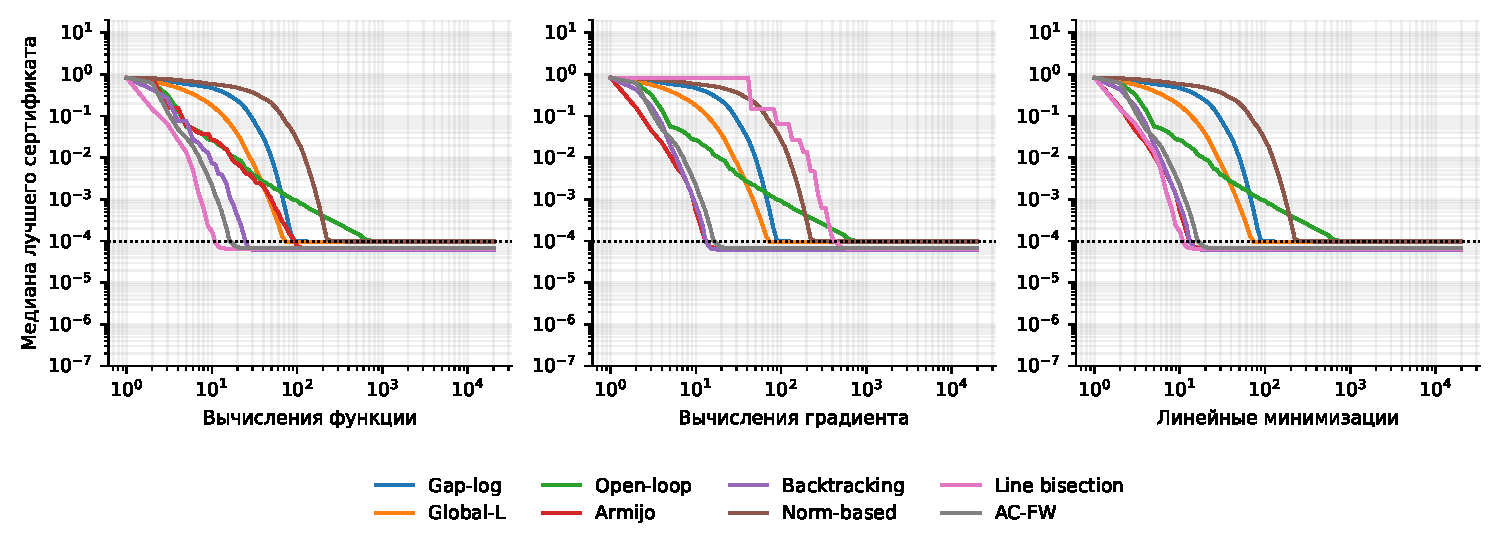
\includegraphics[width=\linewidth]{../figures/multidim_ru.pdf}
\caption{Медиана лучшего записанного сертификата при отдельных
оракульных бюджетах на тех же 54 конфигурациях. После остановки
или исчерпания бюджета сохраняется последнее лучшее значение.
Пунктир соответствует $10^{-4}$. Панели используют разные единицы
стоимости; они не суммируются.}\label{fig:cost_curves}
\end{figure}

\paragraph{Воспроизведение и проверки.}
\texttt{Code/benchmark\_gap.py} воспроизводит исходные проверки,
а \texttt{Code/benchmark\_multidim.py} сохраняет многомерные точки,
параметры, статусы и счётчики оракулов.
\texttt{Code/report\_results.py} строит таблицы и рисунки из готовых
данных без решения новых задач. Аудит 340\,433 записанных точек
проверяет допустимость, согласованность нижних границ с диагностическими
интервалами, применимые оценки спуска и шага, учёт оракулов.
Границы гессиана дополнительно проверяются не более чем в 25 точках
каждого запуска; их глобальное обоснование --- утверждение~\ref{prop:poisson},
а не эта выборочная проверка.
Восемь отдельных тестов проверяют производные конечными разностями,
скалярное неравенство, масштабирование, фактические вызовы интерфейсов,
остановку в начальном минимуме, пробы Армихо, бисекцию и неоптимальность
результата оракула. Проходят и 13 исходных символьных тождеств.
Зависимости и команды приведены в сопровождающем архиве.
